\documentclass{article}

% Language setting
% Replace `english' with e.g. `spanish' to change the document language
\usepackage[french]{babel}
\usepackage[fleqn]{amsmath} % Aligner les équations à gauche


% Set page size and margins
% Replace `letterpaper' with`a4paper' for UK/EU standard size
\usepackage[letterpaper,top=2cm,bottom=2cm,left=3cm,right=3cm,marginparwidth=1.75cm]{geometry}

% Useful packages

\usepackage{amsmath}
\usepackage{graphicx}
\usepackage{subcaption}
\usepackage[colorlinks=true, allcolors=blue]{hyperref}

\title{TD 9 - Equations de Maxwell et ondes élctromagnétiques dans le vide}
\author{IPESUP - PC }
\date{20/10/24}

\begin{document}
\maketitle

\section{Rappels de cours}

\textbf{Equations de Maxwell :}
\begin{align*}
    div(\vec{E}) &= \frac{\rho}{\varepsilon_0} \\
    div(\vec{B}) &= 0 \\
    rot(\vec{E}) &= -\frac{\partial \vec{B}}{\partial t} \\
    rot(\vec{B}) &= \mu_0 \vec{j} + \mu_0 \varepsilon_0 \frac{\partial \vec{E}}{\partial t}\\
\end{align*}

\textbf{Conductivité d'un milieu:}

On définit la conductivité $\gamma$ d'un milieu par la relation $\vec{j} = \gamma \vec{E}$.\\[1cm]



\textbf{Aspect énergétique: }

\begin{enumerate}
  \item Puissance volumique cédée par le champ électromagnétique à la matière : $\mathcal{P}_v = \vec{j} \cdot \vec{E}$
  \item Densité volumique d'énergie électromagnétique : ${u}_{em} = \frac{1}{2}(\varepsilon_0 E^2 + \frac{1}{\mu_0}B^2)$
  \item Vecteur densité de courant d'énergie (ou vecteur de Poynting) : $\vec{\mathcal{\pi}} = \frac{\vec{E} \wedge \vec{B}}{\mu_0}$
  \item Conservation de l'énergie : $\frac{\partial u_{em}}{\partial t} + div(\vec{\mathcal{\pi}}) = -\vec{j} \cdot \vec{E}$ \\[1cm]
\end{enumerate}


\textbf{Ondes électromagnétiques dans le vide: }

Equation de propagation du champ électromagnétique (équation d'Alembert) : $ \Delta \vec{E} - \frac{1}{c^2} \frac{\partial^2 \vec{E}}{\partial t^2} = 0$, avec $c=\frac{1}{\sqrt{\mu_0 \epsilon_0}}$\\


\textbf{Capacités exigibles: }

\begin{enumerate}
  \item Savoir énoncer les équations de Maxwell. 
  \item Lien entre $\vec{j}$ et $\vec{E}$
  \item Puissance volumique cédée par le champ électromagnétique à la matière, densité volumique d'énergie électromagnétique, vecteur densité de courant d'énergie (ou vecteur de Poynting), conservation de l'énergie.
  \item Retrouver l'équation d'Alembert à partir des équations de Maxwell.
\end{enumerate}



\section{Bilan énergétique d'un cylindre conducteur}


On considère un cylindre conducteur ($\gamma$), de rayon $a$, parcouru par un courant $I$ uniforme. 
\begin{enumerate}
  \item Calculer $\vec{j}$ et en déduire $\vec{E}$.
  \item Calculer le champ magnétique dans le conducteur et en déduire la densité volumique d'énergie électromagnétique puis l'énergie électromagnétique totale contenue dans le conducteur. 
  \item Calculer la puissance cédée par le champ électromagnétique au conducteur par effet joule, et en déduire la résistance du conducteur. 
\end{enumerate}

\section{Paradoxe de Feynman: }

On considère un solénoïde semi-infini de rayon $a$, posé sur une plaque pouvant pivoter autour de l'axe $(Oz)$ et parcouru par un courant $ i(t).$, avec $i(t) = I$, pour $t<0$.  
Sur la plaque sont disposées $N$ charges $q>0$ à une distance $b$ de l'axe. 
A $t=0$, on coupe le courant. 
Que se passe-t-il ? 

On donne le rotationnel en coordonnées cylindriques :

$\vec{rot}(\vec{f}) = \left( \frac{1}{r} \frac{\partial f_z}{\partial \theta} - \frac{\partial f_\theta}{\partial z} \right) \vec{e}_r 
+ \left( \frac{\partial f_r}{\partial z} - \frac{\partial f_z}{\partial r} \right) \vec{e}_\theta 
+ \frac{1}{r} \left( \frac{\partial}{\partial r}(r f_\theta) - \frac{\partial f_r}{\partial \theta} \right) \vec{e}_z $\\


\section{Onde électromagnétique dans le vide}

On considère une onde électromagnétique se propageant dans le vide. On la représentation complexe du champ électrique de cette onde : \\



\[
\vec{E} = \left\{
\begin{array}{l}
0 \\
E_0 cos(\frac{\pi y }{a}) exp(i(\omega t - k_0 z)) \\
\underline{\alpha} E_0 sin (\frac{\pi y}{a}) exp(i(\omega t - k_0 z)) \\
\end{array}
\right.
\]

avec $\underline{\alpha}$ un nombre complexe et $k_0$ positif. 

\begin{enumerate}
  \item Déterminer $\underline{\alpha}$ et $k_0$ en fonction de $E_0$, $\omega$, $a$ et $c$. 
  \item Déterminer le champ magnétique $\vec{B}$ associé à cette onde. 
  \item Calculer le vecteur de Poynting et sa valeur moyenne dans le temps. 
  \item Calculer la valeur moyenne dans le temps de la densité volumique d'énergie. 
\end{enumerate}

\section{Situation qu'on rencontre dans la vie de tous les jours}

On considère un cylindre chargé uniformément en surface et pouvant tourner autour de son axe horizontal. 
Une masse M est suspendue au bout d'un fil inextensible enroulé autour du cylindre. 
On lâche la masse, déterminer $\omega(t)$ la vitesse angulaire du cylindre. \\[2cm]


\section{Guide d'ondes rectangulaire}
Quatre plans métalliques parfaitement conducteurs (sur la figure ci-dessous x=0, x=a, y=0,
y=b) délimitent un guide d’onde de longueur infinie suivant Oz, de section droite rectangulaire et dans lequel règne le vide (permitivité $\epsilon_0$, perméabilité $\mu_0$).
On se propose d’étudier la propagation dans ce guide suivant la direction Oz d’une onde
électromagnétique monochromatique de pulsation $\omega$, dont le champ électrique s’écrit :
$\vec{E}=f(x,y)cos(\omega t-k_g z)\vec{u_x}$. Dans cette expression : f désigne une fonction réelle des 
variables y et x, et $ k_g$ est une constante positive. On posera $k_g=\frac{2\pi}{\lambda_g}$, où $\lambda_g$ est  la  "longueur d’onde
guidée" et on notera : $k_0 = \frac{2\pi}{\lambda_0}=\frac{\omega}{c}$

\begin{figure}[h]
  \centering
  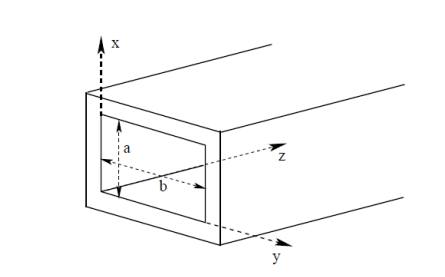
\includegraphics[width=0.4\textwidth]{schéma_guide_d'ondes.png}
  \label{fig:schéma_guide_'ondes}
\end{figure}
\begin{enumerate}
    \item Montrer que $f$ ne dépend que de y puis déterminer l'équation différentielle à laquelle est soumise $f(y)$.
    \item Résoudre cette équation et introduire un entier $n$ correspondant à différents modes propres. 
    \item Déterminer $\vec{B}$.
    \item Exprimer $k_g$ en fonction de $\omega$, c, n et b. En déduire $\lambda_g$ en fonction de $\lambda_0$, b et n.
    \item Montrer qu’il existe une fréquence de coupure $f_c$ en dessous de laquelle il n’y a plus propagation.
    \item Exprimer la vitesse de phase $v_\phi$ de l’onde en fonction de c, n et du rapport $\frac{f}{f_c}$, $f$ étant la fréquence de l'onde.
    \item  Donner l’expression du vecteur de Poynting $\vec{\Pi}$ . Quelle est
    la valeur moyenne  $<\vec{\Pi}>$ dans le temps de ce vecteur ?
    En déduire la puissance moyenne transmise par une section droite du guide d’ondes.
    \item Calculer la valeur moyenne, dans le temps de la densité d’énergie volumique de l’énergie
    électromagnétique $<u>$
    \item A l’aide des résultats précédents, déduire la vitesse de propagation $v_e$ de l’énergie.
    Quelle relation simple peut-on constater entre $v_e $ et $v_\phi$ ? \\[2cm]
\end{enumerate}

\begin{figure}[h]
  \centering
  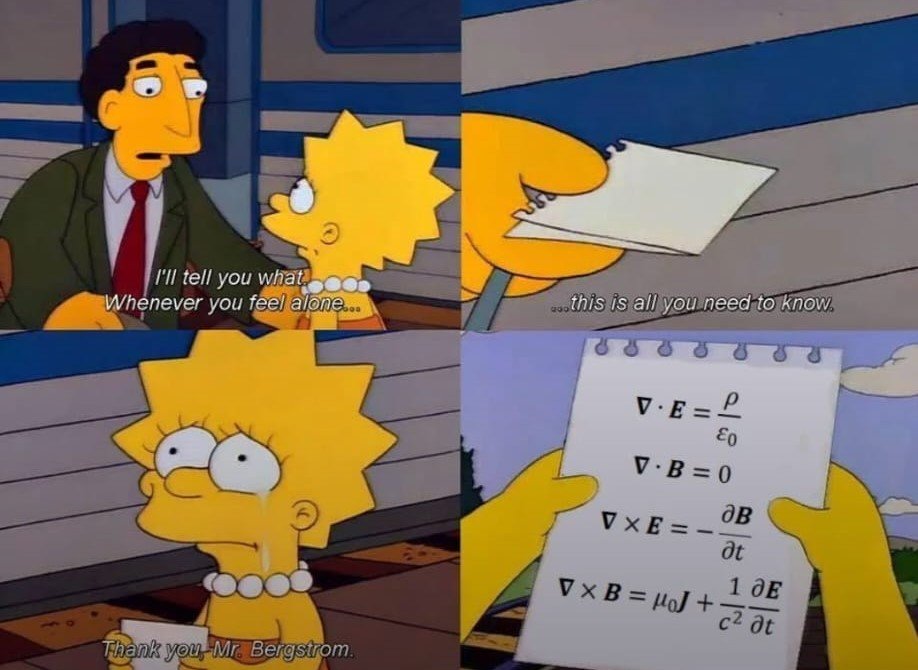
\includegraphics[width=0.5\textwidth]{meme.jpg}
\end{figure}
\end{document}

